\section{问题三：多模态情感预测的层级证据归因}\label{sec:q3}

\subsection{问题分析与总体框架}\label{subsec:q3_overview}
情感预测给出类别与强度，却不能直接说明哪种模态、哪一段有效序列以及哪项输入证据影响了输出。为此，在问题二确定的多模态情感预测模型基础上，本文构建层级式多模态证据归因框架（Hierarchical Evidence Attribution Framework，HEAF）。该框架依次计算模态级精确贡献、模态对交互、连续窗口遮挡效应、删除干预一致性，并把关键槽位连接到经核验的特征来源。总体流程见图~\ref{fig:fig14_q3_heaf_framework}：上部为三模态特征经掩码均值池化与注意力残差池化后的固定预测路径，下部在复用同一预测器的条件下依次分析模态联盟、贡献、交互和关键特征区间；右侧将预测与分层证据组织为解释卡。以下解释的是固定预测函数对输入干预的响应，不直接等同于情绪的现实因果来源。

HEAF由固定预测器、模态联盟归因、连续窗口定位和证据来源映射四级组成。三种模态构成八个完整联盟，以同一预测函数计算分类对数优势与回归输出的精确 Shapley 贡献，并进一步分解模态对交互；随后在主导模态的有效序列上滑动连续窗口，记录遮挡前后的输出差异，再将选中位置与等长随机窗口及分段删除结果比较。文本关键槽位连接至BERT标记和原文字符跨度，音频与视觉关键槽位连接至对应的未对齐特征行。

该层级安排分别回答“哪些模态参与输出”“哪些局部位置对当前预测敏感”以及“关键区间对应哪些特征来源”三个问题。固定预测器和完整联盟使模态贡献可以逐一计算并检查加和关系；连续窗口保留局部序列结构；来源映射使文本、音频、视觉分别获得与其核验结果相符的证据粒度。

\begin{figure}[htbp]
  \centering
  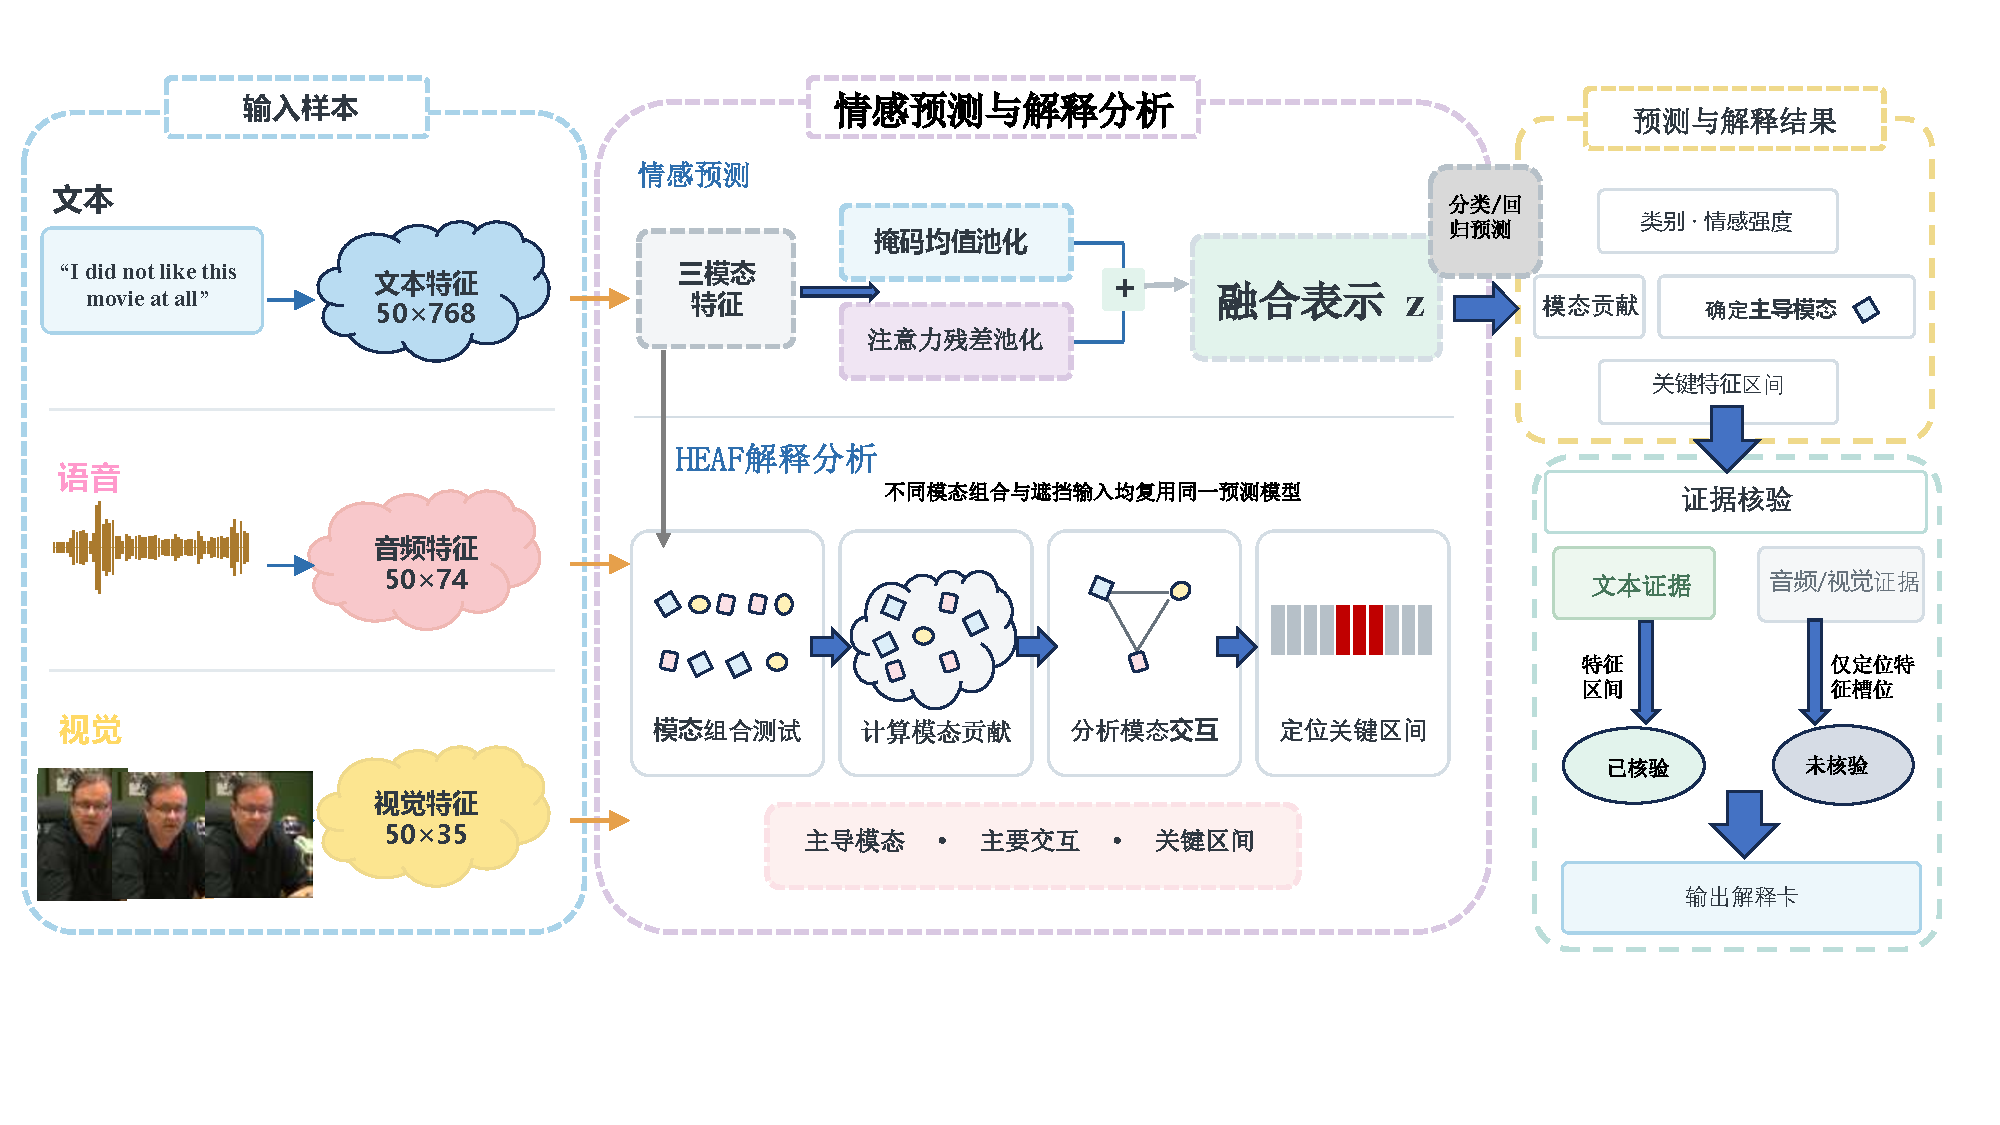
\includegraphics[width=1.0\textwidth]{figures/q3/fig14_q3_heaf_framework.pdf}
  \caption{多模态情感预测与层级证据归因框架。固定预测器给出类别与连续情感强度；HEAF计算模态贡献与交互，并以连续遮挡定位关键特征区间。文本槽位进一步连接原文字符跨度，音频与视觉槽位连接对应的未对齐特征行。图中视频画面和波形为输入上下文示意。}
  \label{fig:fig14_q3_heaf_framework}
\end{figure}

\subsection{模态级精确Shapley归因}\label{subsec:q3_shapley}
三种模态的联盟共有$2^3=8$个，故可逐一计算所有组合，无需采样近似。令$\mathcal M=\{T,A,V\}$，$S\subseteq\mathcal M$ 表示保留的模态集合；未保留模态只在有效位置清零，填充与原生零记录不变。分类解释固定完整输入时预测的类别$c^\star$，以该类别相对其余类别的对数优势为联盟目标：
\begin{equation}
v_{\mathrm c}(S)
=z_{c^\star}(S)-\log\!\sum_{k\ne c^\star}\exp z_k(S),
\qquad
v_{\mathrm r}(S)=\widehat y^{\mathrm r}(S).
\label{eq:q3_value}
\end{equation}
空联盟对应所有有效模态均被清零后的模型输出。对分类或回归目标分别计算
\begin{equation}
\phi_m
=\sum_{S\subseteq\mathcal M\setminus\{m\}}
\frac{|S|!\,(2-|S|)!}{3!}
\bigl[v(S\cup\{m\})-v(S)\bigr].
\label{eq:q3_shapley}
\end{equation}
由此有$\sum_m\phi_m=v(\mathcal M)-v(\varnothing)$，可用作计算完整性检查。分类贡献的单位是对数优势，回归贡献的单位是连续情感强度，两者不可直接混合排序。分类主导模态取最大正贡献；若三者均不为正，则取绝对贡献最大者并标明其非正性质。回归主导模态取绝对贡献最大者；并列时按文本、语音、视觉的固定顺序处理。下述时间分析遵循分类主导模态。
% TODO: add a verified Shapley reference to the bibliography before final submission.

\subsection{模态间交互分析}\label{subsec:q3_interaction}
单个模态贡献之外，本文对文本--语音、文本--视觉和语音--视觉分别计算二阶交互。对模态$i,j$及剩余模态$k$，令
\begin{equation}
\begin{aligned}
I_{ij}=\tfrac12\{&
v(\{i,j\})-v(\{i\})-v(\{j\})+v(\varnothing)\\
&+v(\mathcal M)-v(\{i,k\})-v(\{j,k\})+v(\{k\})\}.
\end{aligned}
\label{eq:q3_interaction}
\end{equation}
该量平均了不含和包含第三模态两种背景下的二阶差分。正值表示联合贡献超过相应加性基准；负值表示联合贡献低于该基准，其具体含义还需结合样本与目标函数解释，不能一概称为冗余。分类和回归仍分别计算交互量。

在附件2验证集728条样本上，两种目标的二阶交互统计见表~\ref{tab:q3_interaction}。分类目标中，文本--语音和语音--视觉的平均交互为负，文本--视觉为正；回归目标中，文本--语音为负，其余两对为正。符号仅描述固定模型的联合输入相对可加和组合的预测贡献。附件4的样本16给出一个较强的个体交互例子，其文本--视觉分类交互为$-0.724$，与总体平均值的方向不同，体现了逐样本解释的必要性。

\begin{table}[htbp]
\centering\small
\caption{附件2验证集分类与回归解释目标的二阶模态交互（$n=728$）}
\label{tab:q3_interaction}
\begin{tabular}{@{}llrrl@{}}
\toprule
解释目标 & 模态对 & 平均交互 & 主要符号比例 & 主要符号\\
\midrule
\multirow{3}{*}{分类} & 文本--语音 & $-0.0706$ & $69.4\%$ & 负\\
 & 文本--视觉 & $+0.0781$ & $60.3\%$ & 正\\
 & 语音--视觉 & $-0.0372$ & $64.4\%$ & 负\\
\addlinespace
\multirow{3}{*}{回归} & 文本--语音 & $-0.1592$ & $85.7\%$ & 负\\
 & 文本--视觉 & $+0.0503$ & $65.4\%$ & 正\\
 & 语音--视觉 & $+0.0592$ & $84.1\%$ & 正\\
\bottomrule
\end{tabular}
\end{table}

\subsection{连续窗口时间遮挡与关键区间定位}\label{subsec:q3_temporal}
模态级归因给出重要模态，却未确定模态序列中的局部位置。对分类主导模态，在有效长度$L_i$内设窗口长度$w_i=\max(1,\operatorname{round}(0.30L_i))$，以步长1遍历所有连续窗口。记$g(\mathbf x)$为式~\eqref{eq:q3_value} 的固定类别对数优势，窗口$W$的遮挡效应为
\begin{equation}
D_i(W)=g(\mathbf x_i)-g\!\left(\mathbf x_i^{\setminus W}\right),
\label{eq:q3_occlusion}
\end{equation}
其中仅该模态在窗口$W$内的有效特征被清零。若存在正效应，取$D_i(W)$最大的窗口；否则取绝对效应最大的窗口并标注方向。平局选择最早位置。覆盖某位置的窗口效应最大值形成50位局部曲线。图中的区间以从零开始的对齐特征槽位表示。对回归报告有符号或绝对输出变化，不预设遮挡使情感强度单向下降。

\subsection{解释忠实性的干预一致性检验}\label{subsec:q3_faithfulness}
问题三复用问题二的固定预测器（seed 42），类别与强度的预测接口保持一致。其在附件2验证集上的基础性能见表~\ref{tab:q3_predictor}。中性类别F1为0.467836、召回率为0.434783，低于另外两类，是主要分类误差来源之一。以下干预统计衡量解释与模型输出变化的一致性，与该表的预测性能含义不同。

\begin{table}[htbp]
\centering\small
\setlength{\tabcolsep}{6pt}
\caption{Q3固定预测器在附件2验证集上的基础性能（seed 42，$n=728$）}
\label{tab:q3_predictor}
\begin{tabular}{@{}cccc@{}}
\toprule
Accuracy & Macro-F1 & MAE & Pearson\\
\midrule
0.648352 & 0.623435 & 0.608260 & 0.646170\\
\midrule
消极F1 & 中性F1 & 积极F1 & 中性召回率\\
\midrule
0.689655 & 0.467836 & 0.712813 & 0.434783\\
\bottomrule
\end{tabular}
\end{table}

时间窗口比例0.30是在附件2验证集的设计子集上确定的。按视频标识分组后，设计子集含332条片段、113个视频标识，独立的审计子集含396条片段、126个视频标识，两组视频标识无交集。审计时把所选窗口与32次随机抽取的等长窗口比较，并按时间曲线删除10\%、20\%、30\%、40\%的有效位置；区间估计采用视频分组自助采样。

表~\ref{tab:q3_faithfulness} 显示，审计子集上所选窗口的平均分类对数优势下降为0.482771，随机窗口为0.082036，差值0.400735，对应分组自助采样95\%区间为$[0.3635,0.4372]$；以每条样本32次随机抽样的均值为对照，所选窗口效应更大的审计样本比例为1.0。置信度下降差为0.077718，类别logit下降差为0.239688。连续回归输出的有符号差为$-0.018095$且区间跨零，但绝对变化差为0.103545。图~\ref{fig:fig15_q3_faithfulness_validation} 同时展示728条验证样本的主导模态分布及审计子集的删除曲线。

\begin{table}[htbp]
\centering\small
\setlength{\tabcolsep}{4pt}
\caption{附件2验证集审计子集的解释干预一致性结果（396条片段；按视频分组的95\%自助采样区间）}
\label{tab:q3_faithfulness}
\begin{tabular}{@{}lcccc@{}}
\toprule
输出量 & 所选窗口 & 随机等长窗口 & 平均差 & 95\%区间\\
\midrule
分类对数优势下降 & 0.482771 & 0.082036 & 0.400735 & $[0.3635,0.4372]$\\
分类置信度下降 & 0.093286 & 0.015567 & 0.077718 & $[0.0712,0.0843]$\\
分类logit下降 & 0.292982 & 0.053294 & 0.239688 & $[0.2195,0.2603]$\\
回归有符号变化 & 0.002082 & 0.020177 & $-0.018095$ & $[-0.0526,0.0141]$\\
回归绝对变化 & 0.202760 & 0.099215 & 0.103545 & $[0.0883,0.1203]$\\
\bottomrule
\end{tabular}
\end{table}

\begin{figure}[htbp]
  \centering
  % TODO: replace with final figure if typography changes in the final manuscript
  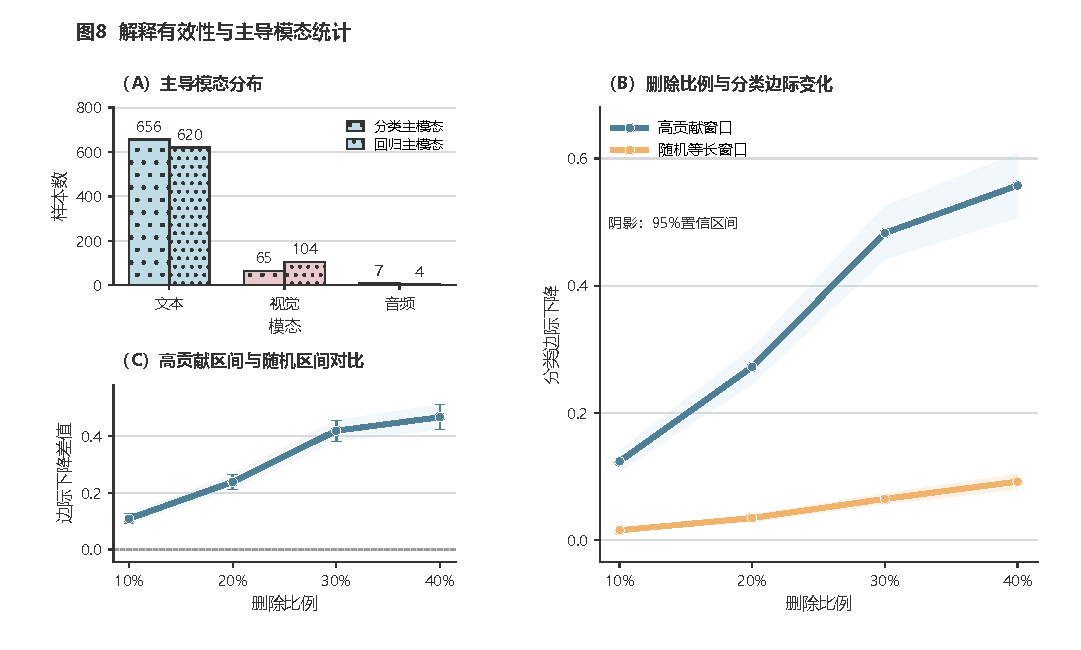
\includegraphics[width=1.0\textwidth]{figures/q3/fig15_q3_faithfulness_validation.pdf}
  \caption{验证集上的主导模态与删除干预结果。（A）728条样本的分类/回归主导模态计数；（B）审计子集上所选与随机窗口的分类边际下降及视频分组95\%区间；（C）两种删除方式的配对差。所选窗口来自同一候选集合的最大影响值，因此相对随机窗口的优势含选择效应。}
  \label{fig:fig15_q3_faithfulness_validation}
\end{figure}

删除10\%、20\%、30\%、40\%有效位置时，所选位置相对随机位置的平均分类边际下降差分别为0.108296、0.237758、0.418076和0.465465。单个关键窗口由候选窗口中的最大影响值确定，故该优势包含选择效应；干预结果表示固定模型的扰动响应一致性，与预测正确率分别解释。固定审计子集上的跨种子解释稳定性见表~\ref{tab:q3_seed_stability}：主导模态与贡献排序整体具有较高一致性，关键区间的位置波动更明显。

\begin{table}[htbp]
\centering\small
\setlength{\tabcolsep}{4pt}
\caption{附件2审计子集的跨种子解释稳定性（seed 42分别与43、44比较；$n=396$）}
\label{tab:q3_seed_stability}
\begin{tabular}{@{}llccc@{}}
\toprule
解释目标 & 种子对 & 主导模态一致率 & Shapley排序相关 & 关键区间IoU\\
\midrule
\multirow{2}{*}{分类} & 42/43 & 0.869 & 0.818 & 0.579\\
 & 42/44 & 0.831 & 0.783 & 0.527\\
\multirow{2}{*}{回归} & 42/43 & 0.778 & 0.745 & ---\\
 & 42/44 & 0.783 & 0.760 & ---\\
\bottomrule
\end{tabular}
\par\vspace{2pt}{\footnotesize 分类排序相关仅统计两种子预测类别一致的样本；区间定位按分类目标定义，回归未单独定义关键区间。}
\end{table}

\subsection{分层证据来源映射}\label{subsec:q3_grounding}
附件4的文本链路连接“对齐特征槽位$\rightarrow$BERT标记$\rightarrow$原文字符区间”。20条样本共604个有效文本槽位的同索引余弦最大值均位于对应行，平均同索引余弦为0.999999994，最大绝对特征差为$3.0041\times10^{-5}$，重构均方根误差为$8.3977\times10^{-7}$。据此，文本主导案例的关键槽位可呈现其原文片段及字符跨度。

音频与视觉采用“对齐特征槽位$\rightarrow$未对齐特征行”的证据层级。附件4中，564/564个非零音频对齐行、534/534个非零视觉对齐行均在对应样本的未对齐特征数组中具有唯一且逐元素相等的行。因而关键区间可进一步给出特征行索引。图~\ref{fig:fig16_q3_case_explanations} 中的视频画面标作“视频上下文示意”，用于呈现对应样本的场景背景。

\subsection{附件4预测解释结果}\label{subsec:q3_attachment4}
依据前述方法对附件4的20条对齐样本生成预测与解释卡。表~\ref{tab:q3_attachment4} 汇总类别、主导模态和证据层级；表~\ref{tab:q3_attachment4_all} 列出全部预测，表~\ref{tab:q3_attachment4_explanations} 列出对应的三模态分类贡献及关键区间。附件4为无标签样本，这些表反映预测与解释分布，不作为预测性能评价。

\begin{table}[htbp]
\centering\small
\caption{附件4的无标签预测及解释摘要（共20条样本）}
\label{tab:q3_attachment4}
\begin{tabular}{@{}llrr@{}}
\toprule
统计项 & 类别或状态 & 数量 & 比例\\
\midrule
\multirow{3}{*}{预测情感类别} & 消极 & 7 & 35\%\\
 & 中性 & 5 & 25\%\\
 & 积极 & 8 & 40\%\\
\addlinespace
\multirow{3}{*}{分类主导模态} & 文本 & 19 & 95\%\\
 & 语音 & 0 & 0\%\\
 & 视觉 & 1 & 5\%\\
\addlinespace
\multirow{3}{*}{回归主导模态} & 文本 & 18 & 90\%\\
 & 语音 & 0 & 0\%\\
 & 视觉 & 2 & 10\%\\
\addlinespace
\multirow{2}{*}{分类主导证据层级} & 原文字符级 & 19 & 95\%\\
 & 未对齐特征行级 & 1 & 5\%\\
\bottomrule
\end{tabular}
\end{table}

\FloatBarrier
\begin{table}[htbp]
\centering\small\setlength{\tabcolsep}{4pt}
\caption{附件4全部20条无标签样本的预测与解释结果；关键区间为从零开始的特征槽位$[a,b)$}
\label{tab:q3_attachment4_all}
\begin{tabular}{@{}llrrlcl@{}}
\toprule
样本ID & 预测类别 & 情感强度 & 置信度 & 分类主导 & 关键区间 & 证据核验\\
\midrule
\texttt{\detokenize{01}} & 中性 & +0.177915 & 0.5359 & 文本 & $[17,24)$ & 文本已核验\\
\texttt{\detokenize{02}} & 消极 & -0.027301 & 0.3898 & 视觉 & $[1,7)$ & 视觉槽位未核验\\
\texttt{\detokenize{03}} & 中性 & -0.064430 & 0.5441 & 文本 & $[0,10)$ & 文本已核验\\
\texttt{\detokenize{04}} & 消极 & -0.398096 & 0.6741 & 文本 & $[20,28)$ & 文本已核验\\
\texttt{\detokenize{05}} & 积极 & +0.886586 & 0.7131 & 文本 & $[0,5)$ & 文本已核验\\
\texttt{\detokenize{06}} & 积极 & +0.759221 & 0.7287 & 文本 & $[14,25)$ & 文本已核验\\
\texttt{\detokenize{07}} & 积极 & +0.799232 & 0.7699 & 文本 & $[13,28)$ & 文本已核验\\
\texttt{\detokenize{08}} & 积极 & +0.678992 & 0.7512 & 文本 & $[8,12)$ & 文本已核验\\
\texttt{\detokenize{09}} & 消极 & -1.987819 & 0.9671 & 文本 & $[2,8)$ & 文本已核验\\
\texttt{\detokenize{10}} & 消极 & -1.556107 & 0.9453 & 文本 & $[21,31)$ & 文本已核验\\
\texttt{\detokenize{11}} & 消极 & -0.965641 & 0.8577 & 文本 & $[1,6)$ & 文本已核验\\
\texttt{\detokenize{12}} & 消极 & -0.981858 & 0.8488 & 文本 & $[31,44)$ & 文本已核验\\
\texttt{\detokenize{13}} & 中性 & +0.173788 & 0.5675 & 文本 & $[0,10)$ & 文本已核验\\
\texttt{\detokenize{14}} & 中性 & +0.154869 & 0.5568 & 文本 & $[1,12)$ & 文本已核验\\
\texttt{\detokenize{15}} & 积极 & +1.267568 & 0.8941 & 文本 & $[14,21)$ & 文本已核验\\
\texttt{\detokenize{16}} & 消极 & -2.030377 & 0.9670 & 文本 & $[8,12)$ & 文本已核验\\
\texttt{\detokenize{17}} & 积极 & +1.656759 & 0.9493 & 文本 & $[9,17)$ & 文本已核验\\
\texttt{\detokenize{18}} & 中性 & -0.158624 & 0.5781 & 文本 & $[6,21)$ & 文本已核验\\
\texttt{\detokenize{19}} & 积极 & +0.276115 & 0.3840 & 文本 & $[29,41)$ & 文本已核验\\
\texttt{\detokenize{20}} & 积极 & +0.875848 & 0.8013 & 文本 & $[0,14)$ & 文本已核验\\
\bottomrule
\end{tabular}
\end{table}

\begin{table}[H]
\centering\small\setlength{\tabcolsep}{3.5pt}
\caption{附件4全部20条样本的分类贡献与证据层级；区间为从零开始的对齐特征槽位$[a,b)$}
\label{tab:q3_attachment4_explanations}
\begin{tabular}{@{}lrrrlcl@{}}
\toprule
ID & $\phi_T$ & $\phi_A$ & $\phi_V$ & 主导模态 & 关键区间 & 证据层级\\
\midrule
\texttt{\detokenize{01}} & +0.4448 & +0.0283 & +0.0097 & 文本 & $[17,24)$ & 原文字符级\\
\texttt{\detokenize{02}} & -0.1971 & +0.2277 & +0.8294 & 视觉 & $[1,7)$ & 特征行级\\
\texttt{\detokenize{03}} & +0.6919 & -0.1267 & -0.0492 & 文本 & $[0,10)$ & 原文字符级\\
\texttt{\detokenize{04}} & +1.9249 & +0.1198 & -0.0096 & 文本 & $[20,28)$ & 原文字符级\\
\texttt{\detokenize{05}} & +1.1092 & -0.3336 & +0.6619 & 文本 & $[0,5)$ & 原文字符级\\
\texttt{\detokenize{06}} & +2.2790 & -0.2529 & -0.5109 & 文本 & $[14,25)$ & 原文字符级\\
\texttt{\detokenize{07}} & +1.6925 & -0.3365 & +0.3790 & 文本 & $[13,28)$ & 原文字符级\\
\texttt{\detokenize{08}} & +2.4908 & -0.2620 & -0.5967 & 文本 & $[8,12)$ & 原文字符级\\
\texttt{\detokenize{09}} & +4.0872 & +0.4352 & +0.1656 & 文本 & $[2,8)$ & 原文字符级\\
\texttt{\detokenize{10}} & +3.6626 & +0.4324 & +0.0621 & 文本 & $[21,31)$ & 原文字符级\\
\texttt{\detokenize{11}} & +2.0970 & +0.2465 & +0.7610 & 文本 & $[1,6)$ & 原文字符级\\
\texttt{\detokenize{12}} & +2.1874 & -0.0032 & +0.8495 & 文本 & $[31,44)$ & 原文字符级\\
\texttt{\detokenize{13}} & +0.5928 & +0.0180 & +0.0000 & 文本 & $[0,10)$ & 原文字符级\\
\texttt{\detokenize{14}} & +1.5361 & +0.0546 & -1.0233 & 文本 & $[1,12)$ & 原文字符级\\
\texttt{\detokenize{15}} & +2.9847 & -0.3149 & -0.0090 & 文本 & $[14,21)$ & 原文字符级\\
\texttt{\detokenize{16}} & +3.8314 & +0.4557 & +0.3986 & 文本 & $[8,12)$ & 原文字符级\\
\texttt{\detokenize{17}} & +3.4202 & -0.1421 & +0.1781 & 文本 & $[9,17)$ & 原文字符级\\
\texttt{\detokenize{18}} & +0.8431 & -0.0933 & -0.0955 & 文本 & $[6,21)$ & 原文字符级\\
\texttt{\detokenize{19}} & +0.6310 & -0.4071 & -0.1692 & 文本 & $[29,41)$ & 原文字符级\\
\texttt{\detokenize{20}} & +2.0873 & -0.2851 & +0.1195 & 文本 & $[0,14)$ & 原文字符级\\
\bottomrule
\end{tabular}
\end{table}

\FloatBarrier

分类与回归的主导模态在17条样本上相同，占85\%。19条文本主导样本对应原文字符级证据；一条视觉主导样本对应未对齐特征行级证据。表中的$\phi$均为分类对数优势目标的Shapley贡献。

\subsection{典型样本分析与本问小结}\label{subsec:q3_cases}
图~\ref{fig:fig16_q3_case_explanations} 展示两条按既定规则选取的案例。样本14为文本主导的原文证据案例：预测类别为中性，连续强度$+0.154869$，分类贡献$\phi_T=+1.536072$、$\phi_A=+0.054570$、$\phi_V=-1.023311$。关键特征区间为$[1,12)$，对应原文字符区间$[0,38)$，原文片段为“He is the co-founder of Rossen and Vet”。

样本02为视觉特征级证据案例：预测类别为消极，连续强度$-0.027301$，分类贡献$\phi_T=-0.197115$、$\phi_A=+0.227718$、$\phi_V=+0.829375$。视觉关键区间$[1,7)$包含从零开始的对齐槽位1--6，逐行对应未对齐视觉特征行36--41。图中的视频画面仅作上下文示意。两个案例共同呈现模态贡献、关键槽位和相应的证据来源。

\begin{figure}[htbp]
  \centering
  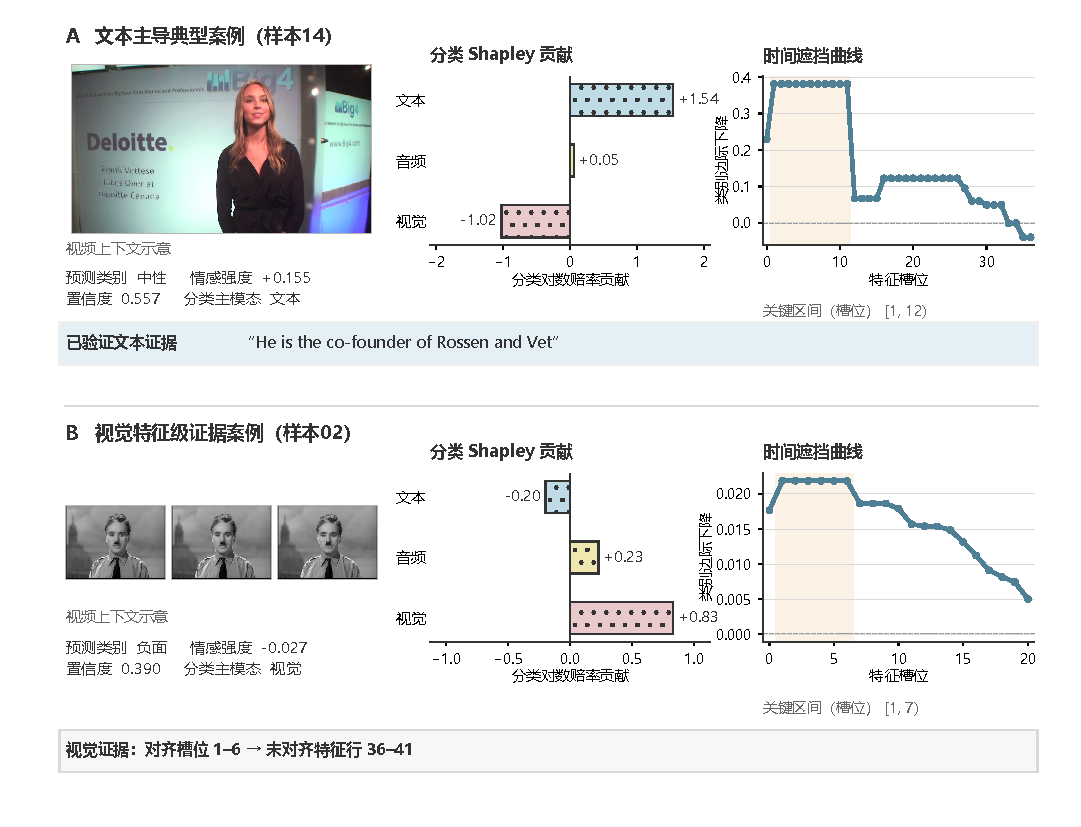
\includegraphics[width=1.0\textwidth]{figures/q3/fig16_q3_case_explanations.pdf}
  \caption{附件4两条典型样本的层级解释。（A）样本14的文本关键槽位映射至原文字符区间；（B）样本02的视觉关键槽位1--6映射至未对齐视觉特征行36--41。视频画面为“视频上下文示意”。}
  \label{fig:fig16_q3_case_explanations}
\end{figure}

本问形成三层解释：模态层以精确Shapley贡献确定文本、语音、视觉的作用及主导模态；区间层以连续遮挡定位对预测敏感的对齐特征区间；证据层将文本区间映射至原文字符片段，将音频与视觉区间映射至未对齐特征行。验证集干预检验支持解释与固定模型输出变化的一致性，附件4给出无标签样本的逐条解释。原始音视频时间位置不纳入本文证据粒度。
\FloatBarrier
